\documentclass{article}
\usepackage[utf8]{inputenc}
\usepackage{enumerate}
\usepackage{enumitem}
\usepackage{float}
\usepackage{graphicx}
\usepackage{multirow, array}
\usepackage[spanish,activeacute]{babel}


\title{Práctica 2: Gestión de una Web de cine}
\author{Rafael Nogales Vaquero
\\Lothar Soto Palma
\\Elena Toro Pérez
\\Jose Ramón Trillo Vilchez}
\date{5 Noviembre del 2014}

\begin{document}

\maketitle

\section{Introducción}
\section{Jerarquia de casos de uso}
\subsection*{Gestión de Usuarios}
	\begin{description}
	\item[Descripción]:\\ Escenarios asociados con la gestión de usuarios, clientes y administradores/empleados.
	\item[Casos de Uso]: 
	\begin{itemize}
		\item Acceder a lista de Almas Gemelas.
		\item Actualizar Películas. 
		\item Añadir/borrar Películas.  %
		\item Banear usuarios.		   %
		\item Comprar Película.			% Falta Caso de Uso
		\item Consulta a Empleado/Administrador. %
		\item Consultar cuenta de Usuario. %
		\item Consultar información de Usuario. %
		\item Consultar películas. %
		\item Control de comentarios/críticas. %
		\item Eliminar cuenta de Usuario. %
		\item Identificar Usuario.		%
		\item Listar usuarios Baneados del sistema.
		\item Listar usuarios colaboradores.
		\item Moderación de usuarios.
		\item Modificar información de Usuario.
		\item Registro(Alta usuario).
\end{itemize}	 
	\item[Actores]:\\ Cliente, Usuario, Administrador, Sistema.
	\end{description}
	
\subsection*{Gestión de Almas Gemelas}
	\begin{description}
	\item[Descripción]:\\ Escenarios asociados con la gestión y formación de almas gemelas.
	\item[Casos de Uso]:
	\begin{itemize}
		\item Acceder a lista de Almas Gemelas.        %
		\item Actualización de lista de Almas Gemelas. %
		\item Asociación de Almas Gemelas.             %
	\end{itemize}		
	\item[Actores]:\\ Usuario, Sistema.
	\end{description}

\subsection*{Gestión de Películas}
	\begin{description}
	\item[Descripción]:\\ Escenarios asociados con el mantenimiento de las fichas de las películas.

	\item[Casos de uso]:
	\begin{itemize}
		\item Añadir imágenes, vídeos, etc de películas.
		\item Añadir películas. 
		\item Borrar películas. 
		\item Comparar película. %  Falta Caso de Uso
		\item Escribir crítica.  %
		\item Listar películas valoradas.
		\item Modificar datos de la película.
		\item Sugerencias de películas a añadir.
		\item Valorar películas.
		\item Ver información.
	\end{itemize}		
	\item[Actores]:\\ Usuario, Sistema, Cliente.
	\end{description}
	
\subsection*{Gestión de Ventas}
	\begin{description}
	\item[Descripción]:\\ Escenarios asociados con la gestión de ventas de películas.
	\item[Casos de Uso]:
	\begin{itemize}
		\item Comprar Película. %Falta Caso de Uso
		\item Disponibilidad de Películas. %
		\item Identificar Usuario.						
		\item Pago a Cuenta.
		\item Pago en Metálico.
		\item Pago con Tarjeta.
		\item Reservar Película.
	\end{itemize}	
	\item[Actores]:\\ Usuario, Administrador.
	\end{description}
	
\section{Diagrama de paquetes}
	\begin{figure}[h]
		\begin{center}
   			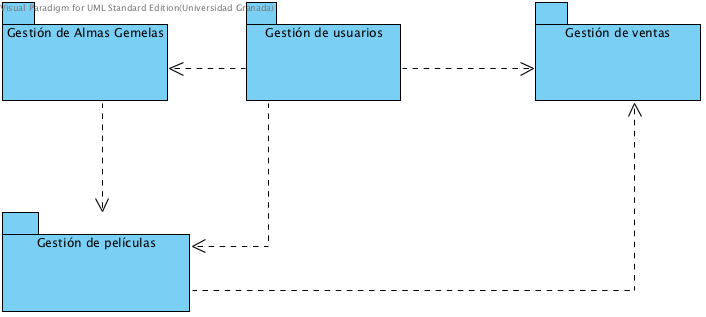
\includegraphics[scale=0.75]{Paquetes.png}
 	  	\end{center}
 	 \end{figure}

\pagebreak

\section{Diagrama de casos de uso}
\subsection*{Gestión de Usuarios, Autor: Lothar Soto Palma}
		\begin{center}
   			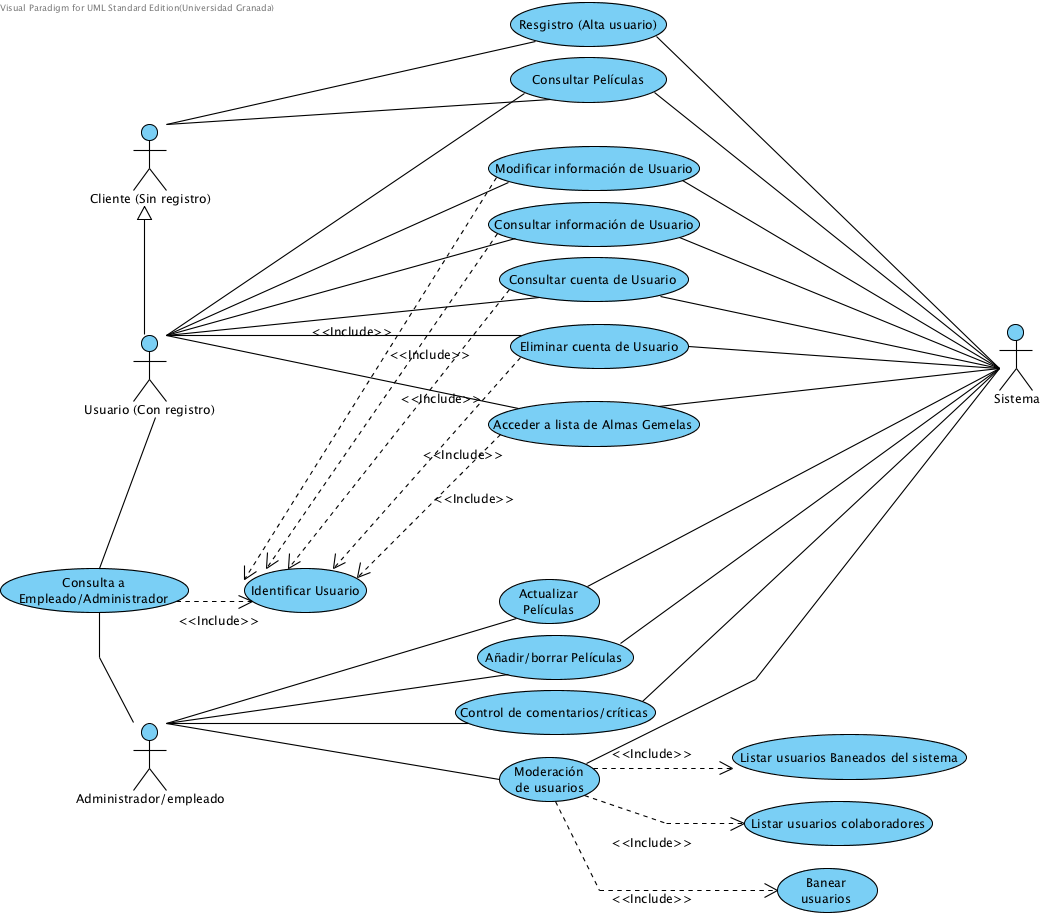
\includegraphics[scale=0.65]{GestiondeUsuarios.png}
   		\end{center}	
   		\pagebreak
\subsection*{Gestión de Almas Gemelas, Autor: Rafael Nogales Vaquero}
		\begin{center}
   			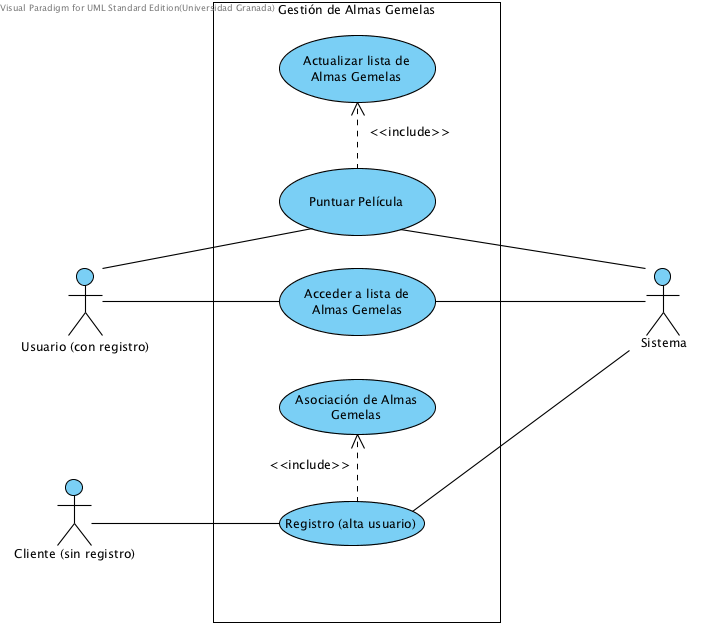
\includegraphics[scale=0.65]{GestiondeAlmasGemelas.png}
   		\end{center}	
   		\pagebreak
\subsection*{Gestión de Películas, Autor: Jose Ramón Trillo Vilchez}
		\begin{center}
   			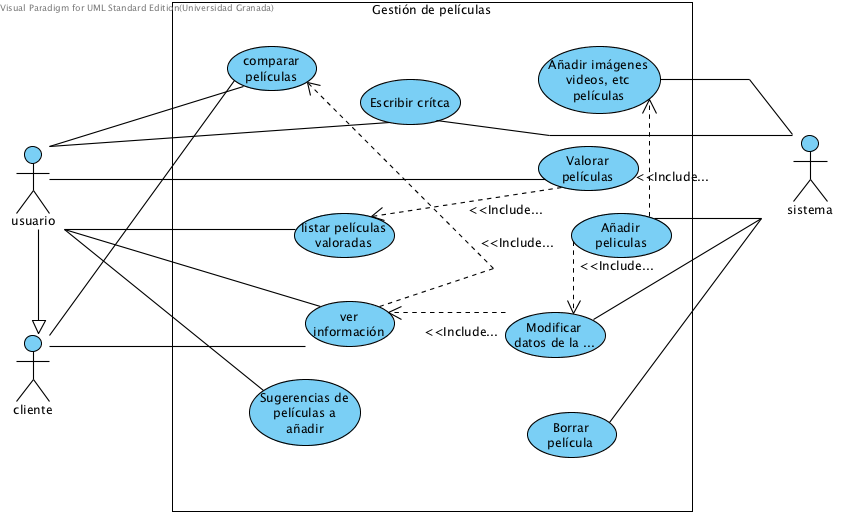
\includegraphics[scale=0.65]{GestiondePeliculas.png}
   		\end{center}	
   		\pagebreak
\subsection*{Gestión de Ventas, Autor: Elena Toro Pérez}
		\begin{center}
   			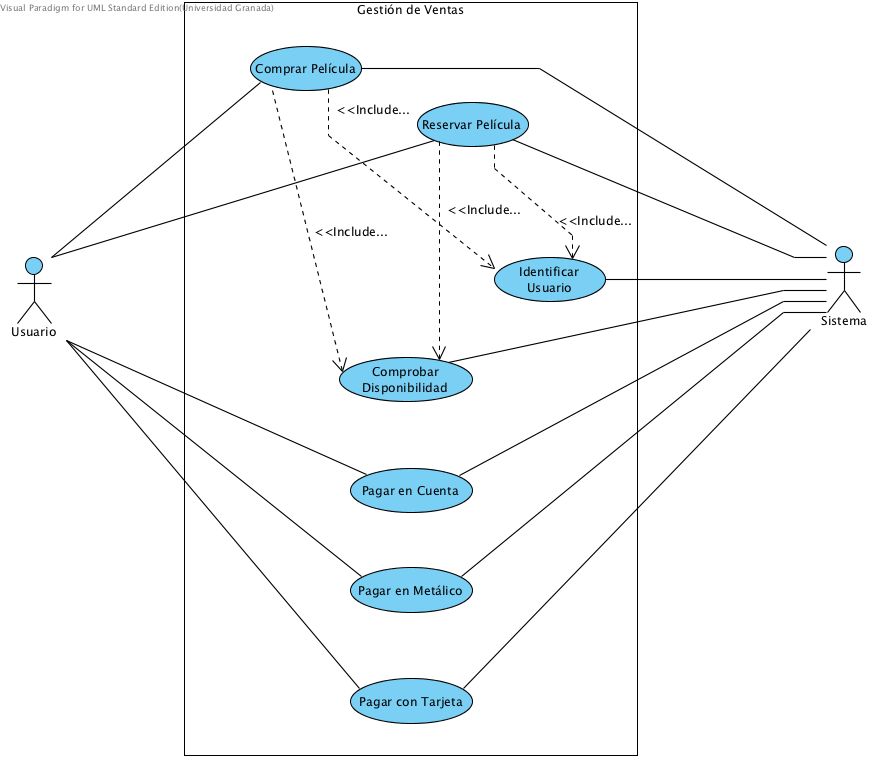
\includegraphics[scale=0.65]{GestiondeVentas.png}
   		\end{center}	
   		\pagebreak
\section{Descripción básica de casos de uso}
%Tablas de Casos de uso:

\begin{table}[h]
\begin{tabular}{|l|l|l|l|l|l|}
\hline
\multicolumn{2}{|p{2cm}|}{Casos de uso}  & \multicolumn{3}{p{7cm}|}{\textbf{Acceder a lista de almas gemelas}} & CU-x \\
\hline
\multicolumn{2}{|p{2cm}|}{Actores}       & \multicolumn{4}{p{8cm}|}{Usuario(Con registro), Sistema}        \\
\hline
\multicolumn{2}{|p{2cm}|}{Tipo}          & \multicolumn{4}{p{8cm}|}{Primario, Esencial}        \\
\hline
\multicolumn{2}{|p{2cm}|}{Precondición}  & \multicolumn{4}{p{8cm}|}{Se debe poseer una cuenta de usuario (registrado).}        \\
\hline
\multicolumn{2}{|p{2cm}|}{Postcondición} & \multicolumn{4}{p{8cm}|}{}        \\
\hline
\multicolumn{6}{|p{10cm}|}{Proposito}                                   \\
\hline
\multicolumn{6}{|p{10cm}|}{Dar a conocer al usuario una serie de personas que tienen los mismos gustos que dicha persona.}                                            \\
\hline
\multicolumn{6}{|p{10cm}|}{Descripción}                                 \\
\hline
\multicolumn{6}{|p{10cm}|}{Permite dar al usuario conocimiento de que personas comparten sus gustos y en parte están relacionadas con él.}                                            \\
\hline
Autor          &       Lothar Soto        & Fecha    &  8/11/14   &   Versión  & 1.0\\    
\hline
\end{tabular}
\end{table}

\begin{table}[h]
\begin{tabular}{|l|l|l|l|l|l|}
\hline
\multicolumn{2}{|p{2cm}|}{Casos de uso}  & \multicolumn{3}{p{7cm}|}{\textbf{Añadir imágenes,videos,etc de películas}} & CU-3 \\
\hline
\multicolumn{2}{|p{2cm}|}{Actores}       & \multicolumn{4}{p{8cm}|}{Sistema}        \\
\hline
\multicolumn{2}{|p{2cm}|}{Tipo}          & \multicolumn{4}{p{8cm}|}{Secundario,Optativo}        \\
\hline
\multicolumn{2}{|p{2cm}|}{Precondición}  & \multicolumn{4}{p{8cm}|}{Que la película esté añadida}        \\
\hline
\multicolumn{2}{|p{2cm}|}{Postcondición} & \multicolumn{4}{p{8cm}|}{}        \\
\hline
\multicolumn{6}{|p{10cm}|}{Proposito}                                   \\
\hline
\multicolumn{6}{|p{10cm}|}{Proporcionar al Usuario información visual sobre la película }                                            \\
\hline
\multicolumn{6}{|p{10cm}|}{Descripción}                                 \\
\hline
\multicolumn{6}{|p{10cm}|}{Es añadir los posters, trailer, imágenes de rodaje de una película que esté añadida}                                            \\
\hline
Autor              &      Jose Ramón Trillo        & Fecha   & 9/11/2014     &   Versión  &1.0\\
\hline
\end{tabular}
\end{table}

\begin{table}[h]
\begin{tabular}{|l|l|l|l|l|l|}
\hline
\multicolumn{2}{|p{2cm}|}{Casos de uso}  & \multicolumn{3}{p{7cm}|}{\textbf{Añadir Películas}} & CU-6 \\
\hline
\multicolumn{2}{|p{2cm}|}{Actores}       & \multicolumn{4}{p{8cm}|}{Sistema}        \\
\hline
\multicolumn{2}{|p{2cm}|}{Tipo}          & \multicolumn{4}{p{8cm}|}{Primario,Esencial}        \\
\hline
\multicolumn{2}{|p{2cm}|}{Precondición}  & \multicolumn{4}{p{8cm}|}{Que la película exista o se vaya a estrenar}        \\
\hline
\multicolumn{2}{|p{2cm}|}{Postcondición} & \multicolumn{4}{p{8cm}|}{}        \\
\hline
\multicolumn{6}{|p{10cm}|}{Proposito}                                   \\
\hline
\multicolumn{6}{|p{10cm}|}{Mantener viva la web y actualizarla con películas nuevas}                                            \\
\hline
\multicolumn{6}{|p{10cm}|}{Descripción}                                 \\
\hline
\multicolumn{6}{|p{10cm}|}{Consiste en añadir la ficha de una película}                                            \\
\hline
Autor              &     Jose Ramón Trillo         & Fecha    &  9/11/2014   &   Versión  &1.0\\
\hline
\end{tabular}
\end{table}

\begin{table}[h]
\begin{tabular}{|l|l|l|l|l|l|}
\hline
\multicolumn{2}{|p{2cm}|}{Casos de uso}  & \multicolumn{3}{p{7cm}|}{\textbf{Actualización de lista de Almas Gemelas}} & CU-x \\
\hline
\multicolumn{2}{|p{2cm}|}{Actores}       & \multicolumn{4}{p{8cm}|}{Usuario, Sistema}        \\
\hline
\multicolumn{2}{|p{2cm}|}{Tipo}          & \multicolumn{4}{p{8cm}|}{Secundario, Esencial}        \\
\hline
\multicolumn{2}{|p{2cm}|}{Precondición}  & \multicolumn{4}{p{8cm}|}{El usuario estaba en lista de espera para actualizar su lista de Almas Gelemas.
Para entrar en la lista de espera basta con haber puntuado $m$ peliculas con $m > $ \textit{umbral de actualización de Almas Gemelas}.}   \\
\hline
\multicolumn{2}{|p{2cm}|}{Postcondición} & \multicolumn{4}{p{8cm}|}{El usuario se saca de la lista de espera para actualizar peliculas (y su contador $m$ se pone a cero).}        \\
\hline
\multicolumn{6}{|p{10cm}|}{Proposito}                                   \\
\hline
\multicolumn{6}{|p{10cm}|}{Conseguir que el usuario tenga asociadas unas Almas Gemelas 
cada vez más afines a sus gustos.}                                            \\
\hline
\multicolumn{6}{|p{10cm}|}{Descripción}                                 \\
\hline
\multicolumn{6}{|p{10cm}|}{Cuando puntuamos una película automaticamente estamos dando información sobre nuestros gustos y el sistema busca entre la lista de usuarios a aquellos que se parecen más a tí en función de tus gustos por lo que la lista se va mejorando con cada puntuación.
\linebreak \linebreak
\textit{Nota: Como el proceso de busqueda de Almas Gemelas es relativamente costoso computacionalmente se puede hacer que el sistema actualice tu lista a la n-esima vez que puntues una película, dónde n es el  ``umbral de actualización de Almas Gemelas``, el cual puede ser inversamente proporcional al cuadrado del número de usuarios del sistema y directamente proporcional a la carga de trabajo del sistema en cada momento, para que de esa forma el sistema esté siempre trabajando pero sea muy dificil que se colapse.}}                                        \\
\hline
Autor              &     Rafael Nogales         & Fecha    &  10/11/14   &   Versión  & 1\\     
\hline
\end{tabular}
\end{table}

\begin{table}[h]
\begin{tabular}{|l|l|l|l|l|l|}
\hline
\multicolumn{2}{|p{2cm}|}{Casos de uso}  & \multicolumn{3}{p{7cm}|}{\textbf{Actualizar Películas}} & CU-x \\
\hline
\multicolumn{2}{|p{2cm}|}{Actores}       & \multicolumn{4}{p{8cm}|}{Administrador/Empleado, Sistema}        \\
\hline
\multicolumn{2}{|p{2cm}|}{Tipo}          & \multicolumn{4}{p{8cm}|}{Primario, Esencial}        \\
\hline
\multicolumn{2}{|p{2cm}|}{Precondición}  & \multicolumn{4}{p{8cm}|}{Necesario tener los permisos de administrador o empleado del sistema.}        \\
\hline
\multicolumn{2}{|p{2cm}|}{Postcondición} & \multicolumn{4}{p{8cm}|}{}        \\
\hline
\multicolumn{6}{|p{10cm}|}{Proposito}                                   \\
\hline
\multicolumn{6}{|p{10cm}|}{Actualizar la lista de películas disponibles.}                                            \\
\hline
\multicolumn{6}{|p{10cm}|}{Descripción}                                 \\
\hline
\multicolumn{6}{|p{10cm}|}{Permite actualizar la lista de películas si anteriormente se ha añadido una o borrado.}                                            \\
\hline
Autor          &       Lothar Soto        & Fecha    &  8/11/14   &   Versión  & 1.0\\    
\hline
\end{tabular}
\end{table}

\begin{table}[h]
\begin{tabular}{|l|l|l|l|l|l|}
\hline
\multicolumn{2}{|p{2cm}|}{Casos de uso}  & \multicolumn{3}{p{7cm}|}{\textbf{Asociación de Almas Gemelas}} & CU-x \\
\hline
\multicolumn{2}{|p{2cm}|}{Actores}       & \multicolumn{4}{p{8cm}|}{Usuario, Sistema}        \\
\hline
\multicolumn{2}{|p{2cm}|}{Tipo}          & \multicolumn{4}{p{8cm}|}{Secundario, Esencial}        \\
\hline
\multicolumn{2}{|p{2cm}|}{Precondición}  & \multicolumn{4}{p{8cm}|}{El usuario acaba de registrarse por primera vez.}        \\
\hline
\multicolumn{2}{|p{2cm}|}{Postcondición} & \multicolumn{4}{p{8cm}|}{}        \\
\hline
\multicolumn{6}{|p{10cm}|}{Proposito}                                   \\
\hline
\multicolumn{6}{|p{10cm}|}{Asociar unas almas gemelas iniciales al cliente recien registrado.}                                            \\
\hline
\multicolumn{6}{|p{10cm}|}{Descripción}                                 \\
\hline
\multicolumn{6}{|p{10cm}|}{El cliente se registra en el sistema y automaticamente se le asocian unas 
almas gemelas inicales basandonos en los gustos del resto de usuarios del sistema, se da un mayor peso a los gustos de usuarios en función de tener la misma nacionalidad, el mismo sexo y una edad cercana a la del cliente.}                                        \\
\hline
Autor              &     Rafael Nogales         & Fecha    &  10/11/14   &   Versión  & 1\\     
\hline
\end{tabular}
\end{table}

\begin{table}[h]
\begin{tabular}{|l|l|l|l|l|l|}
\hline
\multicolumn{2}{|p{2cm}|}{Casos de uso}  & \multicolumn{3}{p{7cm}|}{\textbf{Borrar Películas}} & CU-x \\
\hline
\multicolumn{2}{|p{2cm}|}{Actores}       & \multicolumn{4}{p{8cm}|}{Administrador/Empleado, Sistema}        \\
\hline
\multicolumn{2}{|p{2cm}|}{Tipo}          & \multicolumn{4}{p{8cm}|}{Primario, Esencial}        \\
\hline
\multicolumn{2}{|p{2cm}|}{Precondición}  & \multicolumn{4}{p{8cm}|}{Necesario tener los permisos de administrador o empleado del sistema.}        \\
\hline
\multicolumn{2}{|p{2cm}|}{Postcondición} & \multicolumn{4}{p{8cm}|}{}        \\
\hline
\multicolumn{6}{|p{10cm}|}{Proposito}                                   \\
\hline
\multicolumn{6}{|p{10cm}|}{Conseguir una lista actualizada de películas en el sistema.}                                            \\
\hline
\multicolumn{6}{|p{10cm}|}{Descripción}                                 \\
\hline
\multicolumn{6}{|p{10cm}|}{Permite a los empleados y administradores añadir películas al sistema y borrarlas dependiende de lo que interese.}                                            \\
\hline
Autor          &       Lothar Soto        & Fecha    &  8/11/14   &   Versión  & 1.0\\    
\hline
\end{tabular}
\end{table}

\begin{table}[h]
\begin{tabular}{|l|l|l|l|l|l|}
\hline
\multicolumn{2}{|p{2cm}|}{Casos de uso}  & \multicolumn{3}{p{7cm}|}{\textbf{Banear Usuario}} & CU-x \\
\hline
\multicolumn{2}{|p{2cm}|}{Actores}       & \multicolumn{4}{p{8cm}|}{Administrador/Empleado, Sistema}        \\
\hline
\multicolumn{2}{|p{2cm}|}{Tipo}          & \multicolumn{4}{p{8cm}|}{Secundario, Esencial}        \\
\hline
\multicolumn{2}{|p{2cm}|}{Precondición}  & \multicolumn{4}{p{8cm}|}{Necesario tener los permisos de administrador o empleado del sistema.}        \\
\hline
\multicolumn{2}{|p{2cm}|}{Postcondición} & \multicolumn{4}{p{8cm}|}{}        \\
\hline
\multicolumn{6}{|p{10cm}|}{Proposito}                                   \\
\hline
\multicolumn{6}{|p{10cm}|}{Denegar el acceso a un usuario conflictivo.}                                            \\
\hline
\multicolumn{6}{|p{10cm}|}{Descripción}                                 \\
\hline
\multicolumn{6}{|p{10cm}|}{Permite a los administradores y empleados denegar el acceso a un usuario conflictivo del sistema.}                                            \\
\hline
Autor          &       Lothar Soto        & Fecha    &  8/11/14   &   Versión  & 1.0\\    
\hline
\end{tabular}
\end{table}

\begin{table}[h]
\begin{tabular}{|l|l|l|l|l|l|}
\hline
\multicolumn{2}{|p{2cm}|}{Casos de uso}  & \multicolumn{3}{p{7cm}|}{\textbf{Borrar Película}} & CU-10 \\
\hline
\multicolumn{2}{|p{2cm}|}{Actores}       & \multicolumn{4}{p{8cm}|}{Sistema}        \\
\hline
\multicolumn{2}{|p{2cm}|}{Tipo}          & \multicolumn{4}{p{8cm}|}{Secundario, Esencial}        \\
\hline
\multicolumn{2}{|p{2cm}|}{Precondición}  & \multicolumn{4}{p{8cm}|}{Haya error en la ficha que deteriore o ocupe memoria}        \\
\hline
\multicolumn{2}{|p{2cm}|}{Postcondición} & \multicolumn{4}{p{8cm}|}{}        \\
\hline
\multicolumn{6}{|p{10cm}|}{Proposito}                                   \\
\hline
\multicolumn{6}{|p{10cm}|}{Eliminar películas repetidas que el sistema haya añadido varias veces}                                            \\
\hline
\multicolumn{6}{|p{10cm}|}{Descripción}                                 \\
\hline
\multicolumn{6}{|p{10cm}|}{Consiste en borrar la ficha de una película}                                            \\
\hline
Autor              &      Jose Ramón Trillo        & Fecha    & 9/11/2014    &   Versión  &1.0\\
\hline
\end{tabular}
\end{table}

\begin{table}[h]
\begin{tabular}{|l|l|l|l|l|l|}
\hline
\multicolumn{2}{|p{2cm}|}{Casos de uso}  & \multicolumn{3}{p{7cm}|}{\textbf{Comparar Película}} & CU-1 \\
\hline
\multicolumn{2}{|p{2cm}|}{Actores}       & \multicolumn{4}{p{8cm}|}{Cliente, Usuario}        \\
\hline
\multicolumn{2}{|p{2cm}|}{Tipo}          & \multicolumn{4}{p{8cm}|}{Secundario,Opcional}        \\
\hline
\multicolumn{2}{|p{2cm}|}{Precondición}  & \multicolumn{4}{p{8cm}|}{Tiene que elegir mas de una película}        \\
\hline
\multicolumn{2}{|p{2cm}|}{Postcondición} & \multicolumn{4}{p{8cm}|}{}        \\
\hline
\multicolumn{6}{|p{10cm}|}{Proposito}                                   \\
\hline
\multicolumn{6}{|p{10cm}|}{ver que película nos parece mejor}                                            \\
\hline
\multicolumn{6}{|p{10cm}|}{Descripción}                                 \\
\hline
\multicolumn{6}{|p{10cm}|}{sirve para ver los datos de varias películas a la vez}                                            \\
\hline
Autor              &      Jose Ramón Trillo        & Fecha   & 9/11/2014     &   Versión  &1.0\\
\hline
\end{tabular}
\end{table}

\begin{table}[ht]
\begin{tabular}{|l|l|l|l|l|l|}
\hline
\multicolumn{2}{|p{2cm}|}{Casos de uso}  & \multicolumn{3}{p{7cm}|}{\textbf{Comprar Película}} & CU-x \\
\hline
\multicolumn{2}{|p{2cm}|}{Actores}       & \multicolumn{4}{p{8cm}|}{Usuario(I), Sistema}        \\
\hline
\multicolumn{2}{|p{2cm}|}{Tipo}          & \multicolumn{4}{p{8cm}|}{Primario, Esencial}        \\
\hline
\multicolumn{2}{|p{2cm}|}{Precondición}  & \multicolumn{4}{p{8cm}|}{Las películas para comprar deben estar disponibles para su venta}        \\
\hline
\multicolumn{2}{|p{2cm}|}{Postcondición} & \multicolumn{4}{p{8cm}|}{La venta realizada queda almacenada y se le notifica al usuario sobre ello}        \\
\hline
\multicolumn{6}{|p{10cm}|}{Proposito}                                   \\
\hline
\multicolumn{6}{|p{10cm}|}{Realizar la venta de una película en DVD}                                            \\
\hline
\multicolumn{6}{|p{10cm}|}{Descripción}                                 \\
\hline
\multicolumn{6}{|p{10cm}|}{El usuario se conecta a la página web y, una vez que se ha identificado como socio, elige la película y la opción de comprar en DVD (si existe dicha opción y hay unidades disponibles).
Se almacena la venta, el cliente realiza el pago, en ese momento o posteriormente, y se le proporciona un resguardo mediante e-mail.}                                            \\
\hline
Autor           &Elena Toro              & Fecha    &10-11-14     &   Versión  &1.0\\
\hline
\end{tabular}
\end{table}

\begin{table}[ht]
\begin{tabular}{|l|l|l|l|l|l|}
\hline
\multicolumn{2}{|p{2cm}|}{Casos de uso}  & \multicolumn{3}{p{7cm}|}{Comprobar disponibilidad} & CU-x \\
\hline
\multicolumn{2}{|p{2cm}|}{Actores}       & \multicolumn{4}{p{8cm}|}{Sistema(I)}        \\
\hline
\multicolumn{2}{|p{2cm}|}{Tipo}          & \multicolumn{4}{p{8cm}|}{Primario, Esencial}        \\
\hline
\multicolumn{2}{|p{2cm}|}{Precondición}  & \multicolumn{4}{p{8cm}|}{}        \\
\hline
\multicolumn{2}{|p{2cm}|}{Postcondición} & \multicolumn{4}{p{8cm}|}{Si la película está disponible para su venta en DVD, el socio ya la puede comprar. En otro caso, el socio la podrá reservar si lo desea.}        \\
\hline
\multicolumn{6}{|p{10cm}|}{Proposito}                                   \\
\hline
\multicolumn{6}{|p{10cm}|}{Comprobar la disponibilidad de una película para su venta en DVD.}                                            \\
\hline
\multicolumn{6}{|p{10cm}|}{Descripción}                                 \\
\hline
\multicolumn{6}{|p{10cm}|}{El usuario indica la película a consultar y el sistema comprobará su estado de disponibilidad.}                                            \\
\hline
Autor           &Elena Toro              & Fecha    &10-11-14     &   Versión  &1.0\\
\hline
\end{tabular}
\end{table}

\begin{table}[h]
\begin{tabular}{|l|l|l|l|l|l|}
\hline
\multicolumn{2}{|p{2cm}|}{Casos de uso}  & \multicolumn{3}{p{7cm}|}{\textbf{Consulta a Empleado/Administrador}} & CU-x \\
\hline
\multicolumn{2}{|p{2cm}|}{Actores}       & \multicolumn{4}{p{8cm}|}{Usuario (Con registro), Administrador/Empleado}        \\
\hline
\multicolumn{2}{|p{2cm}|}{Tipo}          & \multicolumn{4}{p{8cm}|}{Primario, Esencial}        \\
\hline
\multicolumn{2}{|p{2cm}|}{Precondición}  & \multicolumn{4}{p{8cm}|}{Se debe poseer una cuenta de usuario (registrado).}        \\
\hline
\multicolumn{2}{|p{2cm}|}{Postcondición} & \multicolumn{4}{p{8cm}|}{}        \\
\hline
\multicolumn{6}{|p{10cm}|}{Proposito}                                   \\
\hline
\multicolumn{6}{|p{10cm}|}{Contactar el usuario con un administrador o empleado.}                                            \\
\hline
\multicolumn{6}{|p{10cm}|}{Descripción}                                 \\
\hline
\multicolumn{6}{|p{10cm}|}{El usuario podrá usar esta funcionalidad para contactar con un administrador para resolver algún tipo de incidencia o duda.}                                            \\
\hline
Autor          &       Lothar Soto        & Fecha    &  8/11/14   &   Versión  & 1.0\\    
\hline
\end{tabular}
\end{table}


\begin{table}[h]
\begin{tabular}{|l|l|l|l|l|l|}
\hline
\multicolumn{2}{|p{2cm}|}{Casos de uso}  & \multicolumn{3}{p{7cm}|}{\textbf{Consultar cuenta de Usuario}} & CU-x \\
\hline
\multicolumn{2}{|p{2cm}|}{Actores}       & \multicolumn{4}{p{8cm}|}{Usuario (Con registro), Sistema}        \\
\hline
\multicolumn{2}{|p{2cm}|}{Tipo}          & \multicolumn{4}{p{8cm}|}{Primario, Esencial}        \\
\hline
\multicolumn{2}{|p{2cm}|}{Precondición}  & \multicolumn{4}{p{8cm}|}{Se debe poseer una cuenta de usuario (registrado).}        \\
\hline
\multicolumn{2}{|p{2cm}|}{Postcondición} & \multicolumn{4}{p{8cm}|}{}        \\
\hline
\multicolumn{6}{|p{10cm}|}{Proposito}                                   \\
\hline
\multicolumn{6}{|p{10cm}|}{Poder consultar su información agregada en el momento del registro.}                                            \\
\hline
\multicolumn{6}{|p{10cm}|}{Descripción}                                 \\
\hline
\multicolumn{6}{|p{10cm}|}{Permite a los usuarios consultar sus datos de cuenta en caso de olvido como el Correo, o contraseña(Este último requiere confirmación).}                                            \\
\hline
Autor             &     Lothar Soto          & Fecha    &  8/11/14   &   Versión  &1.0\\     
\hline
\end{tabular}
\end{table}


\begin{table}[h]
\begin{tabular}{|l|l|l|l|l|l|}
\hline
\multicolumn{2}{|p{2cm}|}{Casos de uso}  & \multicolumn{3}{p{7cm}|}{\textbf{Consultar información de Usuario}} & CU-x \\
\hline
\multicolumn{2}{|p{2cm}|}{Actores}       & \multicolumn{4}{p{8cm}|}{Usuario (Con registro), Sistema}        \\
\hline
\multicolumn{2}{|p{2cm}|}{Tipo}          & \multicolumn{4}{p{8cm}|}{Primario, Esencial}        \\
\hline
\multicolumn{2}{|p{2cm}|}{Precondición}  & \multicolumn{4}{p{8cm}|}{Debe ser un Usuario por lo que se tiene que estar registrado previamente.}        \\
\hline
\multicolumn{2}{|p{2cm}|}{Postcondición} & \multicolumn{4}{p{8cm}|}{}        \\
\hline
\multicolumn{6}{|p{10cm}|}{Proposito}                                   \\
\hline
\multicolumn{6}{|p{10cm}|}{Conseguir la comodidad con los datos del usuario y que este pueda consultarlos en cualquier momento.}                                            \\
\hline
\multicolumn{6}{|p{10cm}|}{Descripción}                                 \\
\hline
\multicolumn{6}{|p{10cm}|}{El usuario consulta su información de cuenta como el estado,gustos...}                                            \\
\hline
Autor              &     Lothar Soto         & Fecha    &  8/11/14   &   Versión  & 1.0\\     
\hline
\end{tabular}
\end{table}


\begin{table}[h]
\begin{tabular}{|l|l|l|l|l|l|}
\hline
\multicolumn{2}{|p{2cm}|}{Casos de uso}  & \multicolumn{3}{p{7cm}|}{\textbf{Consultar Películas}} & CU-x \\
\hline
\multicolumn{2}{|p{2cm}|}{Actores}       & \multicolumn{4}{p{8cm}|}{Cliente (Sin registro),Usuario(Con registro) , Sistema}        \\
\hline
\multicolumn{2}{|p{2cm}|}{Tipo}          & \multicolumn{4}{p{8cm}|}{Primario, Esencial}        \\
\hline
\multicolumn{2}{|p{2cm}|}{Precondición}  & \multicolumn{4}{p{8cm}|}{}        \\
\hline
\multicolumn{2}{|p{2cm}|}{Postcondición} & \multicolumn{4}{p{8cm}|}{}        \\
\hline
\multicolumn{6}{|p{10cm}|}{Proposito}                                   \\
\hline
\multicolumn{6}{|p{10cm}|}{Que se pueda acceder a información y multimedia hacerca de una película.}                                            \\
\hline
\multicolumn{6}{|p{10cm}|}{Descripción}                                 \\
\hline
\multicolumn{6}{|p{10cm}|}{Permite a los clientes, usuarios acceder a informcación acerca de la película buscada.}                                            \\
\hline
Autor              &     Lothar Soto         & Fecha    &  8/11/14   &   Versión  & 1\\     
\hline
\end{tabular}
\end{table}

\begin{table}[h]
\begin{tabular}{|l|l|l|l|l|l|}
\hline
\multicolumn{2}{|p{2cm}|}{Casos de uso}  & \multicolumn{3}{p{7cm}|}{\textbf{Control de comentarios/críticas}} & CU-x \\
\hline
\multicolumn{2}{|p{2cm}|}{Actores}       & \multicolumn{4}{p{8cm}|}{Administrador/Empleado, Sistema}        \\
\hline
\multicolumn{2}{|p{2cm}|}{Tipo}          & \multicolumn{4}{p{8cm}|}{Primario, Esencial}        \\
\hline
\multicolumn{2}{|p{2cm}|}{Precondición}  & \multicolumn{4}{p{8cm}|}{Necesario tener los permisos de administrador o empleado del sistema.}        \\
\hline
\multicolumn{2}{|p{2cm}|}{Postcondición} & \multicolumn{4}{p{8cm}|}{}        \\
\hline
\multicolumn{6}{|p{10cm}|}{Proposito}                                   \\
\hline
\multicolumn{6}{|p{10cm}|}{Controlar los comentarios de los usuarios puesto pueden resultar inapropiados.}                                            \\
\hline
\multicolumn{6}{|p{10cm}|}{Descripción}                                 \\
\hline
\multicolumn{6}{|p{10cm}|}{Permite a los empleados y administradores  manejar los comentarios (pueden eliminarlos).}                                            \\
\hline
Autor          &       Lothar Soto        & Fecha    &  8/11/14   &   Versión  & 1.0\\    
\hline
\end{tabular}
\end{table}



%%%%%%%%%%%% %%%%%%%%%%%% %%%%%%%% %%%%%%%%%%%% %%
%												%
%    Aquí va el de Disponibilidad De Peliculas	%
%												%
%%%%%%%%%%%% %%%%%%%%%%%% %%%%%%%% %%%%%%%%%%%% %%


\begin{table}[h]
\begin{tabular}{|l|l|l|l|l|l|}
\hline
\multicolumn{2}{|p{2cm}|}{Casos de uso}  & \multicolumn{3}{p{7cm}|}{\textbf{Eliminar cuenta de Usuario}} & CU-x \\
\hline
\multicolumn{2}{|p{2cm}|}{Actores}       & \multicolumn{4}{p{8cm}|}{Usuario(Con registro), Sistema}        \\
\hline
\multicolumn{2}{|p{2cm}|}{Tipo}          & \multicolumn{4}{p{8cm}|}{Primario, Esencial}        \\
\hline
\multicolumn{2}{|p{2cm}|}{Precondición}  & \multicolumn{4}{p{8cm}|}{Se debe poseer una cuenta de usuario (registrado).}        \\
\hline
\multicolumn{2}{|p{2cm}|}{Postcondición} & \multicolumn{4}{p{8cm}|}{}        \\
\hline
\multicolumn{6}{|p{10cm}|}{Proposito}                                   \\
\hline
\multicolumn{6}{|p{10cm}|}{Dar de baja a un usuario y posteriormente eliminar su cuenta.}                                            \\
\hline
\multicolumn{6}{|p{10cm}|}{Descripción}                                 \\
\hline
\multicolumn{6}{|p{10cm}|}{Permite al usuario dejar de usar el sistema sin que quede información de este en el mismo.}                                            \\
\hline
Autor          &       Lothar Soto        & Fecha    &  8/11/14   &   Versión  & 1.0\\     
\hline
\end{tabular}
\end{table}

\clearpage
\begin{table}[h]
\begin{tabular}{|l|l|l|l|l|l|}
\hline
\multicolumn{2}{|p{2cm}|}{Casos de uso}  & \multicolumn{3}{p{7cm}|}{\textbf{Escribir crítica}} & CU-2 \\
\hline
\multicolumn{2}{|p{2cm}|}{Actores}       & \multicolumn{4}{p{8cm}|}{Sistema, Usuario}        \\
\hline
\multicolumn{2}{|p{2cm}|}{Tipo}          & \multicolumn{4}{p{8cm}|}{Primario,Esencial}        \\
\hline
\multicolumn{2}{|p{2cm}|}{Precondición}  & \multicolumn{4}{p{8cm}|}{El cliente esté registrado}        \\
\hline
\multicolumn{2}{|p{2cm}|}{Postcondición} & \multicolumn{4}{p{8cm}|}{}        \\
\hline
\multicolumn{6}{|p{10cm}|}{Proposito}                                   \\
\hline
\multicolumn{6}{|p{10cm}|}{Las personas den su opinión sobre una película}                                            \\
\hline
\multicolumn{6}{|p{10cm}|}{Descripción}                                 \\
\hline
\multicolumn{6}{|p{10cm}|}{Es una opinión subjetiva sobre película visualizada}                                            \\
\hline
Autor              &      Jose Ramón Trillo        & Fecha    & 9/11/2014    &   Versión  &1.0\\
\hline
\end{tabular}
\end{table}

\begin{table}[h]
\begin{tabular}{|l|l|l|l|l|l|}
\hline
\multicolumn{2}{|p{2cm}|}{Casos de uso}  & \multicolumn{3}{p{7cm}|}{\textbf{Identificar Usuario}} & CU-x \\
\hline
\multicolumn{2}{|p{2cm}|}{Actores}       & \multicolumn{4}{p{8cm}|}{Usuario (Con registro), Sistema}        \\
\hline
\multicolumn{2}{|p{2cm}|}{Tipo}          & \multicolumn{4}{p{8cm}|}{Secundario, Esencial}        \\
\hline
\multicolumn{2}{|p{2cm}|}{Precondición}  & \multicolumn{4}{p{8cm}|}{Se debe poseer una cuenta de usuario (registrado).}        \\
\hline
\multicolumn{2}{|p{2cm}|}{Postcondición} & \multicolumn{4}{p{8cm}|}{El usuario identificado como socio ya puede usar la opción de comprar película (o reservarla en su defecto)}        \\
\hline
\multicolumn{6}{|p{10cm}|}{Proposito}                                   \\
\hline
\multicolumn{6}{|p{10cm}|}{Proporcionar una identidad a un usuario en el sistema.}                                            \\
\hline
\multicolumn{6}{|p{10cm}|}{Descripción}                                 \\
\hline
\multicolumn{6}{|p{10cm}|}{El sistema solicita la identificación del usuario como socio mediante su nombre de usuario y contraseña. El sistema comprueba la vericidad de los datos sobre el socio y permite la opción deseada (compra o reserva).}                                            \\
\hline
Autor           &Elena Toro              & Fecha    &10-11-14     &   Versión  &1.0\\    
\hline
\end{tabular}
\end{table}

\begin{table}[h]
\begin{tabular}{|l|l|l|l|l|l|}
\hline
\multicolumn{2}{|p{2cm}|}{Casos de uso}  & \multicolumn{3}{p{7cm}|}{\textbf{Lista de películas valoradas}} & CU-5 \\
\hline
\multicolumn{2}{|p{2cm}|}{Actores}       & \multicolumn{4}{p{8cm}|}{Usuario}        \\
\hline
\multicolumn{2}{|p{2cm}|}{Tipo}          & \multicolumn{4}{p{8cm}|}{Secundario,Esencial}        \\
\hline
\multicolumn{2}{|p{2cm}|}{Precondición}  & \multicolumn{4}{p{8cm}|}{El usuario esté registrado y hya valorado varias películas}        \\
\hline
\multicolumn{2}{|p{2cm}|}{Postcondición} & \multicolumn{4}{p{8cm}|}{}        \\
\hline
\multicolumn{6}{|p{10cm}|}{Proposito}                                   \\
\hline
\multicolumn{6}{|p{10cm}|}{Saber que películas ha valorado el usuario para no repetir}                                            \\
\hline
\multicolumn{6}{|p{10cm}|}{Descripción}                                 \\
\hline
\multicolumn{6}{|p{10cm}|}{Es un listado de películas que el usuario ha valorado a lo largo de su vida como usuario de la web}                                            \\
\hline
Autor              &       Jose Ramón Trillo       & Fecha    & 9/11/2014     &   Versión  &1.0\\
\hline
\end{tabular}
\end{table}


\begin{table}[h]
\begin{tabular}{|l|l|l|l|l|l|}
\hline
\multicolumn{2}{|p{2cm}|}{Casos de uso}  & \multicolumn{3}{p{7cm}|}{\textbf{Listar Usuarios Baneados del sistema}} & CU-x \\
\hline
\multicolumn{2}{|p{2cm}|}{Actores}       & \multicolumn{4}{p{8cm}|}{Administrador/Empleado, Sistema}        \\
\hline
\multicolumn{2}{|p{2cm}|}{Tipo}          & \multicolumn{4}{p{8cm}|}{Secundario, Esencial}        \\
\hline
\multicolumn{2}{|p{2cm}|}{Precondición}  & \multicolumn{4}{p{8cm}|}{Necesario tener los permisos de administrador o empleado del sistema.}        \\
\hline
\multicolumn{2}{|p{2cm}|}{Postcondición} & \multicolumn{4}{p{8cm}|}{}        \\
\hline
\multicolumn{6}{|p{10cm}|}{Proposito}                                   \\
\hline
\multicolumn{6}{|p{10cm}|}{Obtener una lista de los usuarios baneados del sistema.}                                            \\
\hline
\multicolumn{6}{|p{10cm}|}{Descripción}                                 \\
\hline
\multicolumn{6}{|p{10cm}|}{Permite al administrador conocer los usuarios baneados.}                                            \\
\hline
Autor          &       Lothar Soto        & Fecha    &  8/11/14   &   Versión  & 1.0\\    
\hline
\end{tabular}
\end{table}

\begin{table}[h]
\begin{tabular}{|l|l|l|l|l|l|}
\hline
\multicolumn{2}{|p{2cm}|}{Casos de uso}  & \multicolumn{3}{p{7cm}|}{\textbf{Listar Usuarios Colaboradores}} & CU-x \\
\hline
\multicolumn{2}{|p{2cm}|}{Actores}       & \multicolumn{4}{p{8cm}|}{Administrador/Empleado, Sistema}        \\
\hline
\multicolumn{2}{|p{2cm}|}{Tipo}          & \multicolumn{4}{p{8cm}|}{Secundario, Esencial}        \\
\hline
\multicolumn{2}{|p{2cm}|}{Precondición}  & \multicolumn{4}{p{8cm}|}{Necesario tener los permisos de administrador o empleado del sistema.}        \\
\hline
\multicolumn{2}{|p{2cm}|}{Postcondición} & \multicolumn{4}{p{8cm}|}{}        \\
\hline
\multicolumn{6}{|p{10cm}|}{Proposito}                                   \\
\hline
\multicolumn{6}{|p{10cm}|}{Obtener una liste de los usuarios que colaboraron en el sistema.}                                            \\
\hline
\multicolumn{6}{|p{10cm}|}{Descripción}                                 \\
\hline
\multicolumn{6}{|p{10cm}|}{Permite al administrador conocer a los usuarios colaboradores.}                                            \\
\hline
Autor          &       Lothar Soto        & Fecha    &  8/11/14   &   Versión  & 1.0\\    
\hline
\end{tabular}
\end{table}

\begin{table}[h]
\begin{tabular}{|l|l|l|l|l|l|}
\hline
\multicolumn{2}{|p{2cm}|}{Casos de uso}  & \multicolumn{3}{p{7cm}|}{\textbf{Moderación de Usuarios}} & CU-x \\
\hline
\multicolumn{2}{|p{2cm}|}{Actores}       & \multicolumn{4}{p{8cm}|}{Administrador/Empleado, Sistema}        \\
\hline
\multicolumn{2}{|p{2cm}|}{Tipo}          & \multicolumn{4}{p{8cm}|}{Primario, Esencial}        \\
\hline
\multicolumn{2}{|p{2cm}|}{Precondición}  & \multicolumn{4}{p{8cm}|}{Necesario tener los permisos de administrador o empleado del sistema.}        \\
\hline
\multicolumn{2}{|p{2cm}|}{Postcondición} & \multicolumn{4}{p{8cm}|}{}        \\
\hline
\multicolumn{6}{|p{10cm}|}{Proposito}                                   \\
\hline
\multicolumn{6}{|p{10cm}|}{Controlar el comportamiento de los usuarios en el sistema.}                                            \\
\hline
\multicolumn{6}{|p{10cm}|}{Descripción}                                 \\
\hline
\multicolumn{6}{|p{10cm}|}{Permite a los empleados y administradores controlar a los usuarios usando un métodos de sanciones.}                                            \\
\hline
Autor          &       Lothar Soto        & Fecha    &  8/11/14   &   Versión  & 1.0\\    
\hline
\end{tabular}
\end{table}

\begin{table}[h]
\begin{tabular}{|l|l|l|l|l|l|}
\hline
\multicolumn{2}{|p{2cm}|}{Casos de uso}  & \multicolumn{3}{p{7cm}|}{\textbf{Modificar datos de una película}} & CU-8 \\
\hline
\multicolumn{2}{|p{2cm}|}{Actores}       & \multicolumn{4}{p{8cm}|}{Sistema}        \\
\hline
\multicolumn{2}{|p{2cm}|}{Tipo}          & \multicolumn{4}{p{8cm}|}{Primario. Esencial}        \\
\hline
\multicolumn{2}{|p{2cm}|}{Precondición}  & \multicolumn{4}{p{8cm}|}{La película que se va a modificar sea la correcta}        \\
\hline
\multicolumn{2}{|p{2cm}|}{Postcondición} & \multicolumn{4}{p{8cm}|}{Que los datos sean correctos}        \\
\hline
\multicolumn{6}{|p{10cm}|}{Proposito}                                   \\
\hline
\multicolumn{6}{|p{10cm}|}{Cambiar información debido a que es errónea o esté incompleta}                                            \\
\hline
\multicolumn{6}{|p{10cm}|}{Descripción}                                 \\
\hline
\multicolumn{6}{|p{10cm}|}{Es el cambio de información en la ficha de una película}                                            \\
\hline
Autor              &     Jose Ramón Trillo         & Fecha    & 9/11/2014    &   Versión  &1.0\\
\hline
\end{tabular}
\end{table}

\begin{table}[h]
\begin{tabular}{|l|l|l|l|l|l|}
\hline
\multicolumn{2}{|p{2cm}|}{Casos de uso}  & \multicolumn{3}{p{7cm}|}{\textbf{Modificar información de Usuario}} & CU-x \\
\hline
\multicolumn{2}{|p{2cm}|}{Actores}       & \multicolumn{4}{p{8cm}|}{Usuario (Con registro), Sistema}        \\
\hline
\multicolumn{2}{|p{2cm}|}{Tipo}          & \multicolumn{4}{p{8cm}|}{Primario, Esencial}        \\
\hline
\multicolumn{2}{|p{2cm}|}{Precondición}  & \multicolumn{4}{p{8cm}|}{Debe ser un Usuario por lo que se tiene que estar registrado previamente.}        \\
\hline
\multicolumn{2}{|p{2cm}|}{Postcondición} & \multicolumn{4}{p{8cm}|}{}        \\
\hline
\multicolumn{6}{|p{10cm}|}{Proposito}                                   \\
\hline
\multicolumn{6}{|p{10cm}|}{Conseguir la comodidad con los datos del usuario y que este puede modificarlos dentro de ciertas limitaciones.}                                            \\
\hline
\multicolumn{6}{|p{10cm}|}{Descripción}                                 \\
\hline
\multicolumn{6}{|p{10cm}|}{El usuario modifica su información de cuenta como el Correo, Contraseaña...}                                            \\
\hline
Autor              &     Lothar Soto         & Fecha    &  8/11/14   &   Versión  & 1.0\\     
\hline
\end{tabular}
\end{table}

\begin{table}[ht]
\begin{tabular}{|l|l|l|l|l|l|}
\hline
\multicolumn{2}{|p{2cm}|}{Casos de uso}  & \multicolumn{3}{p{7cm}|}{Pagar en Cuenta} & CU-x \\
\hline
\multicolumn{2}{|p{2cm}|}{Actores}       & \multicolumn{4}{p{8cm}|}{Socio(I), Sistema}        \\
\hline
\multicolumn{2}{|p{2cm}|}{Tipo}          & \multicolumn{4}{p{8cm}|}{Secundario, Esencial}        \\
\hline
\multicolumn{2}{|p{2cm}|}{Precondición}  & \multicolumn{4}{p{8cm}|}{}        \\
\hline
\multicolumn{2}{|p{2cm}|}{Postcondición} & \multicolumn{4}{p{8cm}|}{}        \\
\hline
\multicolumn{6}{|p{10cm}|}{Proposito}                                   \\
\hline
\multicolumn{6}{|p{10cm}|}{Acción por parte de un socio de hacer un pago en la cuenta corriente de la web.}                                            \\
\hline
\multicolumn{6}{|p{10cm}|}{Descripción}                                 \\
\hline
\multicolumn{6}{|p{10cm}|}{El socio notifica al sistema de que quiere realizar el pago en la cuenta, indicando la cantidad que desea ingresar y la forma de pago que usará. El sistema verificará el ingreso.}                                            \\
\hline
Autor           &Elena Toro              & Fecha    &10-11-14     &   Versión  &1.0\\
\hline
\end{tabular}
\end{table}

\begin{table}[ht]
\begin{tabular}{|l|l|l|l|l|l|}
\hline
\multicolumn{2}{|p{2cm}|}{Casos de uso}  & \multicolumn{3}{p{7cm}|}{Pagar en Metálico} & CU-x \\
\hline
\multicolumn{2}{|p{2cm}|}{Actores}       & \multicolumn{4}{p{8cm}|}{Socio(I), Sistema}        \\
\hline
\multicolumn{2}{|p{2cm}|}{Tipo}          & \multicolumn{4}{p{8cm}|}{Secundario, Esencial}        \\
\hline
\multicolumn{2}{|p{2cm}|}{Precondición}  & \multicolumn{4}{p{8cm}|}{}        \\
\hline
\multicolumn{2}{|p{2cm}|}{Postcondición} & \multicolumn{4}{p{8cm}|}{}        \\
\hline
\multicolumn{6}{|p{10cm}|}{Proposito}                                   \\
\hline
\multicolumn{6}{|p{10cm}|}{Acción por parte de un socio de pagar en metálico una cantidad determinada.}                                            \\
\hline
\multicolumn{6}{|p{10cm}|}{Descripción}                                 \\
\hline
\multicolumn{6}{|p{10cm}|}{El socio notifica al sistema de que quiere realizar el pago en metálico y el sistema le indica la cantidad a pagar.}                                            \\
\hline
Autor           &Elena Toro              & Fecha    &10-11-14     &   Versión  &1.0\\
\hline
\end{tabular}
\end{table}

\begin{table}[ht]
\begin{tabular}{|l|l|l|l|l|l|}
\hline
\multicolumn{2}{|p{2cm}|}{Casos de uso}  & \multicolumn{3}{p{7cm}|}{Pagar con Tarjeta} & CU-x \\
\hline
\multicolumn{2}{|p{2cm}|}{Actores}       & \multicolumn{4}{p{8cm}|}{Socio(I), Sistema}        \\
\hline
\multicolumn{2}{|p{2cm}|}{Tipo}          & \multicolumn{4}{p{8cm}|}{Secundario, Esencial}        \\
\hline
\multicolumn{2}{|p{2cm}|}{Precondición}  & \multicolumn{4}{p{8cm}|}{}        \\
\hline
\multicolumn{2}{|p{2cm}|}{Postcondición} & \multicolumn{4}{p{8cm}|}{}        \\
\hline
\multicolumn{6}{|p{10cm}|}{Proposito}                                   \\
\hline
\multicolumn{6}{|p{10cm}|}{Acción por parte de un socio de pagar con tarjeta una cantidad determinada.}                                            \\
\hline
\multicolumn{6}{|p{10cm}|}{Descripción}                                 \\
\hline
\multicolumn{6}{|p{10cm}|}{El socio notifica al sistema de que quiere realizar el pago usando una tarjeta de crédito. El sistema le indica la cantidad a pagar,la información necesaria para efectuarlo y almacena la información sobre dicho pago}                                            \\
\hline
Autor           &Elena Toro              & Fecha    &10-11-14     &   Versión  &1.0\\
\hline
\end{tabular}
\end{table}


\begin{table}[h]
\begin{tabular}{|l|l|l|l|l|l|}
\hline
\multicolumn{2}{|p{2cm}|}{Casos de uso}  & \multicolumn{3}{p{7cm}|}{\textbf{Registro(Alta usuario)}} & CU-x \\
\hline
\multicolumn{2}{|p{2cm}|}{Actores}       & \multicolumn{4}{p{8cm}|}{Cliente (Sin registro), Sistema}        \\
\hline
\multicolumn{2}{|p{2cm}|}{Tipo}          & \multicolumn{4}{p{8cm}|}{Primario, Esencial}        \\
\hline
\multicolumn{2}{|p{2cm}|}{Precondición}  & \multicolumn{4}{p{8cm}|}{El cliente no debe poseer cuenta y por tanto no tiene un registro en el sistema.}        \\
\hline
\multicolumn{2}{|p{2cm}|}{Postcondición} & \multicolumn{4}{p{8cm}|}{}        \\
\hline
\multicolumn{6}{|p{10cm}|}{Proposito}                                   \\
\hline
\multicolumn{6}{|p{10cm}|}{Registrar a los clientes sin cuenta en el sistema.}                                            \\
\hline
\multicolumn{6}{|p{10cm}|}{Descripción}                                 \\
\hline
\multicolumn{6}{|p{10cm}|}{El cliente se registra en el sistema para acceder a las opciones del sistema de la que solo pueden hacer uso los usuarios(con registro).}                                            \\
\hline
Autor              &     Lothar Soto         & Fecha    &  8/11/14   &   Versión  & 1\\     
\hline
\end{tabular}
\end{table}

\begin{table}[ht]
\begin{tabular}{|l|l|l|l|l|l|}
\hline
\multicolumn{2}{|p{2cm}|}{Casos de uso}  & \multicolumn{3}{p{7cm}|}{Reservar Película} & CU-x \\
\hline
\multicolumn{2}{|p{2cm}|}{Actores}       & \multicolumn{4}{p{8cm}|}{Usuario(I), Sistema}        \\
\hline
\multicolumn{2}{|p{2cm}|}{Tipo}          & \multicolumn{4}{p{8cm}|}{Primario, Esencial}        \\
\hline
\multicolumn{2}{|p{2cm}|}{Precondición}  & \multicolumn{4}{p{8cm}|}{Las películas a reservar no están disponibles para su venta en DVD}        \\
\hline
\multicolumn{2}{|p{2cm}|}{Postcondición} & \multicolumn{4}{p{8cm}|}{Las películas reservadas se almacenan en una lista ordenada}        \\
\hline
\multicolumn{6}{|p{10cm}|}{Proposito}                                   \\
\hline
\multicolumn{6}{|p{10cm}|}{Reservar una película y ser informado cuando esté disponible para su venta en DVD}                                            \\
\hline
\multicolumn{6}{|p{10cm}|}{Descripción}                                 \\
\hline
\multicolumn{6}{|p{10cm}|}{El usuario se conecta a la página web y, una vez que se ha identificado como socio, elige la película. Al no estar disponible para la compra en DVD, pulsa la opción de reservar, almacenándose el pedido en una lista ordenada.}                                            \\
\hline
Autor           &Elena Toro              & Fecha    &10-11-14     &   Versión  &1.0\\
\hline
\end{tabular}
\end{table}


\begin{table}[h]
\begin{tabular}{|l|l|l|l|l|l|}
\hline
\multicolumn{2}{|p{2cm}|}{Casos de uso}  & \multicolumn{3}{p{7cm}|}{\textbf{Sugerencias de películas a añadir}} & CU-9 \\
\hline
\multicolumn{2}{|p{2cm}|}{Actores}       & \multicolumn{4}{p{8cm}|}{Usuario}        \\
\hline
\multicolumn{2}{|p{2cm}|}{Tipo}          & \multicolumn{4}{p{8cm}|}{Secundario,Opcional}        \\
\hline
\multicolumn{2}{|p{2cm}|}{Precondición}  & \multicolumn{4}{p{8cm}|}{Estar registrado en la web}        \\
\hline
\multicolumn{2}{|p{2cm}|}{Postcondición} & \multicolumn{4}{p{8cm}|}{}        \\
\hline
\multicolumn{6}{|p{10cm}|}{Proposito}                                   \\
\hline
\multicolumn{6}{|p{10cm}|}{Ayudar al sistema a añadir fichas sobre películas que no está añadidas}                                            \\
\hline
\multicolumn{6}{|p{10cm}|}{Descripción}                                 \\
\hline
\multicolumn{6}{|p{10cm}|}{Es una petición del usuario al Sistema para que este añada ficha de alguna película que no se encuentre en la base de datos}                                            \\
\hline
Autor              &    Jose Ramón Trillo         & Fecha    &  9/11/2014   &   Versión  &1.0\\
\hline
\end{tabular}
\end{table}

\begin{table}[h]
\begin{tabular}{|l|l|l|l|l|l|}
\hline
\multicolumn{2}{|p{2cm}|}{Casos de uso}  & \multicolumn{3}{p{7cm}|}{\textbf{Valorar Películas}} & CU-4 \\
\hline
\multicolumn{2}{|p{2cm}|}{Actores}       & \multicolumn{4}{p{8cm}|}{Usuario}        \\
\hline
\multicolumn{2}{|p{2cm}|}{Tipo}          & \multicolumn{4}{p{8cm}|}{Primario,Esencial}        \\
\hline
\multicolumn{2}{|p{2cm}|}{Precondición}  & \multicolumn{4}{p{8cm}|}{El Usuario esté registrado}        \\
\hline
\multicolumn{2}{|p{2cm}|}{Postcondición} & \multicolumn{4}{p{8cm}|}{}        \\
\hline
\multicolumn{6}{|p{10cm}|}{Proposito}                                   \\
\hline
\multicolumn{6}{|p{10cm}|}{El Usuario de una puntuación a la película}                                            \\
\hline
\multicolumn{6}{|p{10cm}|}{Descripción}                                 \\
\hline
\multicolumn{6}{|p{10cm}|}{Es la manera (aparate de las críticas) con la que el usuario puede decir si le ha gustado una película }                                            \\
\hline
Autor              &      Jose Ramón Trillo        & Fecha    & 9/11/2014    &   Versión  &1.0\\
\hline
\end{tabular}
\end{table}

\begin{table}[h]
\begin{tabular}{|l|l|l|l|l|l|}
\hline
\multicolumn{2}{|p{2cm}|}{Casos de uso}  & \multicolumn{3}{p{7cm}|}{\textbf{Ver información de la película}} & CU-7 \\
\hline
\multicolumn{2}{|p{2cm}|}{Actores}       & \multicolumn{4}{p{8cm}|}{Usuario, Cliente}        \\
\hline
\multicolumn{2}{|p{2cm}|}{Tipo}          & \multicolumn{4}{p{8cm}|}{Primario, Esencial}        \\
\hline
\multicolumn{2}{|p{2cm}|}{Precondición}  & \multicolumn{4}{p{8cm}|}{Que la película exista}        \\
\hline
\multicolumn{2}{|p{2cm}|}{Postcondición} & \multicolumn{4}{p{8cm}|}{}        \\
\hline
\multicolumn{6}{|p{10cm}|}{Proposito}                                   \\
\hline
\multicolumn{6}{|p{10cm}|}{proporcionar a la persona datos relevantes sobre la película que consulta}                                            \\
\hline
\multicolumn{6}{|p{10cm}|}{Descripción}                                 \\
\hline
\multicolumn{6}{|p{10cm}|}{Conjunto de datos sobre una película, guardados en la ficha de esta }                                            \\
\hline
Autor              &     Jose Ramón Trillo         & Fecha    & 9/11/2014    &   Versión  &1.0\\
\hline
\end{tabular}
\end{table}

\begin{table}[h]
\begin{tabular}{|l|l|l|l|l|l|}
\hline
\multicolumn{2}{|p{2cm}|}{Casos de uso}  & \multicolumn{3}{p{7cm}|}{\textbf{Votar Películas}} & CU-x \\
\hline
\multicolumn{2}{|p{2cm}|}{Actores}       & \multicolumn{4}{p{8cm}|}{Usuario(Con registro), Sistema}        \\
\hline
\multicolumn{2}{|p{2cm}|}{Tipo}          & \multicolumn{4}{p{8cm}|}{Primario, Esencial}        \\
\hline
\multicolumn{2}{|p{2cm}|}{Precondición}  & \multicolumn{4}{p{8cm}|}{Se debe poseer una cuenta de usuario (registrado).}        \\
\hline
\multicolumn{2}{|p{2cm}|}{Postcondición} & \multicolumn{4}{p{8cm}|}{}        \\
\hline
\multicolumn{6}{|p{10cm}|}{Proposito}                                   \\
\hline
\multicolumn{6}{|p{10cm}|}{Dar la opinión de los usuarios sobre las películas a modo de voto.}                                            \\
\hline
\multicolumn{6}{|p{10cm}|}{Descripción}                                 \\
\hline
\multicolumn{6}{|p{10cm}|}{Permite al usuario votar una película positiva o negativamente.
\linebreak \textit{Nota: Como consecuencia se entra en la lista de espera para actualizar lista de almas gemelas en el caso de que el usuario no estuviese ya en ella.}}                                            \\
\hline
Autor          &       Lothar Soto        & Fecha    &  8/11/14   &   Versión  & 1.0\\     
\hline
\end{tabular}
\end{table}

\end{document}
